\documentclass{jknotes}
\usepackage{joshkirklin,pgfplots}

\newcommand{\dunder}[1]{\underline{\underline{#1}}}
\newcommand{\x}{\bm{x}}
\newcommand{\inv}[1]{\frac{1}{#1}}

\begin{document}

\institution{Cambridge Part III Maths}
\title{Slow Viscous Flow}
\lecturer{John Lister}
\notetaker{Charles Powell}
\date{Michaelmas 2020}

\maketitle
\suggestionsspiel
\tableofcontents

\section{Basic Fluid Mechanics}
\lecture{09/10/20}
`Infinitesimal' fluid particles have well-defined density $\rho(\bm{x},t)$,
velocity $\bm{u}(\bm{x},t)$ and pressure $p(\bm{x},t)$ where $\bm{x}(t)$ is
the position of the fluid particles.

\begin{defn}
	The \emph{Eulerian} or \emph{material} derivative
	\begin{equation}
		\frac{\diffD}{\diffD{t}} = \frac{\partial}{\partial t} + \bm{u}\cdot
		\nabla
	\end{equation}
	is the rate of change following the fluid particle.
\end{defn}

\subsection{Mass Conservation}
In general, we have
\begin{equation}
\frac{\partial \rho}{\partial t} + \nabla \cdot \left(\rho \bm{u}\right) = 0
\iff \frac{\diffD{\rho}}{\diffD{t}} + \rho \nabla \cdot \bm{u} = 0
\end{equation}

For an incompressible fluid, $\frac{\diffD{\rho}}{\diffD{t}} = 0 \iff \nabla
\cdot \bm{u} = 0$

\subsection{The Stress Tensor}
The \emph{stress} $\bm{\tau}$ is the force per unit area acting across a
surface. Force balance on an `infinitesimal' fluid tetahedron shows that the
stress $\bm{\tau}$ is linearly related to the surface normal $\bm{n}$:
\begin{equation}
	\bm{\tau} = \sigma \cdot \bm{n}
\end{equation}
where $\sigma$ is the \emph{stress tensor} and $\bm{\tau}$ is stress exerted
by the outside fluid on the inside of a surface with outward normal $\bm{n}$.
Angular momentum balance shows that $\sigma$ is symmetric in most fluids.

\subsection{Momentum equation}
The \emph{Cauchy momentum equation} states in general
\begin{equation}
	\frac{\diffD{\bm{u}}}{\diffD{t}} = \bm{F} + \nabla \cdot \sigma
\end{equation}

\subsection{Energy equation}
In the case of an incompressible fluid, the rate of local inertial
\emph{viscous dissipation} is derived by contracting the Cauchy momentum
equation with the fluid velocity and integrating over a volume. We have
\begin{equation}
	\mathcal{D} = \int_V e_{ij} \sigma_{ij} \,\diffd{V} = \int_V e:\sigma \,
	\diffd{V}
\end{equation}
where $e_{ij} = \frac{1}{2}\left(\nabla \bm{u} + \left(\nabla
\bm{u}\right)^T\right)$ is the \emph{rate of strain} tensor. Note $e_{ii} = 0$
by incompressibility and $e_{ij} = e_{ji}$. 

The rate of working by external surface forces on the fluid is
\begin{equation}
	\int_{\partial V} u_i \sigma_{ij} n_j \diffd{S}
\end{equation}

\subsection{Newtonian Fluids}
\begin{defn}
Fluid deformation produces internal viscous stresses. If the relationship
between fluid deformation $\frac{\partial u_i}{\partial x_j}$ and stress
$\sigma_{ij}$ is local, linear, instantaneous and isotropic, then the fluid is
\emph{Newtonian}.
\end{defn}

If the fluid is also incompressible, then the stress tensor takes the form
\begin{equation}
	\sigma_{ij} = -p \delta_{ij} + 2\mu e_{ij}
\end{equation}
where $\mu$ is the \emph{dynamic viscosity} and $2 \mu e_{ij}$ is the
\emph{deviatoric stress}. Note that there is no dependence on the vorticity
$\bm{\omega} = \nabla \times \bm{u}$.

For an incompressible Newtonian fluid with uniform viscosity we have the
\emph{Navier-Stokes equations}
\begin{equation}
	\begin{aligned}
		\rho \frac{\diffD{\bm{u}}}{\diffD{t}} &= - \nabla p + \bm{F} + \mu
			\nabla^2 \bm{u} \\
			\nabla \cdot \bm{u} &=0
	\end{aligned}
\end{equation}

The rate of viscous dissipation is
\begin{equation}
	\mathcal{D} = 2 \mu \int e_{ij} e_{ij} \, \diffd{V}
\end{equation}

Often body forces are conservative $\bm{F} = -\nabla \phi$ and we incorporate
$\bm{F}$ into a \emph{modified pressure} $p + \phi$.

\subsection{Boundary conditions}
Kinematic boundary conditions on a fluid-fluid interface are
\begin{itemize}
	\item $\left[ \bm{u} \cdot \bm{n} \right]^+_- = 0$ by mass conservation
	\item $\left[ \bm{u} \times \bm{n} \right]^+_- = \bm{0}$ to avoid infinite
		stresses
\end{itemize}

Kinematic boundary conditions on a rigid boundary are
\begin{itemize}
	\item No flux: $\bm{u} \cdot \bm{n} = 0$
	\item No slip: $\bm{u} \times \bm{n} = \bm{0}$
\end{itemize}

Dynamic boundary conditions in the absence of surface tension are 
\begin{equation}
	\left[\sigma \cdot \bm{n}\right]^+_- = \bm{0}
\end{equation}
Note that modified pressure should not be used here.

With surface tension included, the condition becomes
\begin{equation}
	\left[ \sigma \cdot \bm{n} \right]^+_- = \gamma \kappa \bm{n} - \nabla_s
	\gamma
\end{equation}
where $\kappa = \nabla_s \cdot \bm{n}$ is the \emph{curvature} and $\gamma$ is
the \emph{surface tension}.

\subsection{Reynolds number}
Suppose $U, L, L/U$ are representative velocity, length, and time scales of
the flow. Then
\begin{equation}
	\begin{aligned}
		\rho \frac{\diffD{\bm{u}}}{\diffD{t}} &\sim \rho \frac{U^2}{L} \\
		\mu \nabla^2 \bm{u} &\sim \mu \frac{U}{L^2}
	\end{aligned}
\end{equation}

\begin{defn}
The \emph{Reynolds number} is the ratio of these quantities and determines the
important of inertial vs. viscous stresses. 
\begin{equation}
	\text{Re} = \frac{\rho U L}{\mu} = \frac{U L}{\nu}
\end{equation}
\end{defn}

If $\text{Re} \ll 1$ then inertia is negligible and we have the \emph{Stokes
equations}
\begin{equation}
	\begin{aligned}
		\mu \nabla^2 \bm{u} &= \nabla p - \bm{F} \\
		\nabla \cdot \bm{u} &= 0
	\end{aligned}
\end{equation}

Stokes equations are useful in many regimes.
\begin{itemize}
	\item Large $\mu$, e.g. magma, glass, ice sheets
	\item Small $L$, e.g. microorganisms, microfluid devices
	\item Thin film flows, e.g. lubrication theory
\end{itemize}
\lecture{12/10/20}
\begin{eg}
	Sperm cell -- intrinsic length scales $L \sim 5 \mu m, U \sim 100 \mu m
	\cdot s^{-1}, \nu \sim 10^{-2} cm^2 \cdot s^{-1} = 10^6 \mu m^2 \cdot
	s^{-1}$. Therefore $Re \sim 5 \times 10^{-4}$ so can be described by the
	Stokes equations.
\end{eg}

\begin{eg}
	Mantle convection -- intrinsic length scales $L \sim 1000 km = 10^8 cm, U
	\sim 2 cm \text{year}^{-1} \sim 10^7 cm \cdot s^{-1}, \nu \sim 10^{21}
	cm^2 \cdot s^{-1}$. Thus $Re \sim 10^{-20}$.
\end{eg}

There are some caveats which come with the use of intrinsic length scales.
\begin{itemize}
	\item $\bm{u} \cdot \nabla$ and $\nabla^2$ may not involve the same length
		scale $L$, e.g. in lubrication theory there is a short length scale
		for the depth of the flow, which is small compared to other length
		scales of the flow.
	\item $L$ may vary in the flow e.g. in the far field of a moving body $Re
		\sim \frac{Ur}{\nu}$.
	\item $T$ may not equal $L/U$ if there is an external time scale, e.g.
		oscillating body with $T \sim \omega^{-1}$.
\end{itemize}

\section{The Stokes Equations}
\begin{equation}
	\begin{aligned}
		\nabla \cdot \sigma &= \mu \nabla^2 \bm{u} - \nabla p = - \bm{F} \\
		\nabla \cdot \bm{u} &= 0
	\end{aligned}
\end{equation}

\subsection{Simple Properties}
\subsubsection{Instantaneous}
The Stokes equations involve no $\partial_t$ term, so there is no inertia, no
memory, and the flow only `knows' about the current boundary conditions and
applied forces, and responds immediately to changes. With moving boundaries
(i.e. changing boundary conditions) the flow is \emph{quasi-steady}.

\subsubsection{Linear}
The Stokes equations are linear in $\bm{F}, p$, and $\bm{u}$. Therefore the
fluid response is proportional to forcing and solutions for a given geometry
can be superposed.

\subsubsection{Reversible}
If all the forces change sign, then $\bm{u}$ changes sign. Thus if we reverse
all the forces and the history of their application, the flow returns to its
original state. Reversibility can sometimes be used with a symmetry to rule
out certain behaviours of the flow.

\begin{eg}
	Sedimenting sphere -- consider a sphere sedimenting in a Stokes flow next
	to a rigid wall. Will the sphere migrate laterally?\\
	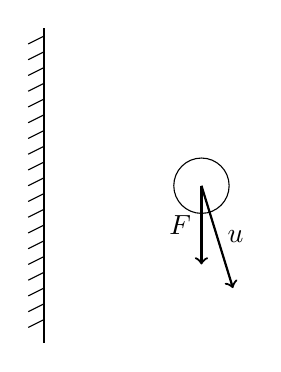
\begin{tikzpicture}
		\draw (-2,2) -- (-2,-2);
		\draw (-2.2, 1.8) -- (-2, 1.9);
		\draw (-2.2, 1.6) -- (-2, 1.7);
		\draw (-2.2, 1.4) -- (-2, 1.5);
		\draw (-2.2, 1.2) -- (-2, 1.3);
		\draw (-2.2, 1) -- (-2, 1.1);
		\draw (-2.2, 0.8) -- (-2, 0.9);
		\draw (-2.2, 0.6) -- (-2, 0.7);
		\draw (-2.2, 0.4) -- (-2, 0.5);
		\draw (-2.2, 0.2) -- (-2, 0.3);
		\draw (-2.2, 0) -- (-2, 0.1);
		\draw (-2.2,-1.8) -- (-2,- 1.7);
		\draw (-2.2,-1.6) -- (-2,- 1.5);
		\draw (-2.2,-1.4) -- (-2,- 1.3);
		\draw (-2.2,-1.2) -- (-2,- 1.1);
		\draw (-2.2,-1.0) -- (-2,- 0.9);
		\draw (-2.2,-0.8) -- (-2,- 0.7);
		\draw (-2.2,-0.6) -- (-2,- 0.5);
		\draw (-2.2,-0.4) -- (-2,- 0.3);
		\draw (-2.2,-0.2) -- (-2,- 0.1);
		\draw (0,0) circle (10pt);
		\draw [->,thick] (0,0) -- (0.4,-1.3) node[right, midway] {$\bm{u}$};
		\draw [->, thick] (0,0) -- (0,-1) node[left, midway] {$\bm{F}$};
	\end{tikzpicture}

	Applying reversibility, change $\bm{F} \to -\bm{F}$ so $\bm{u} \to
	-\bm{u}$:\\
	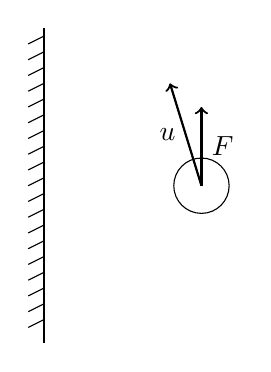
\begin{tikzpicture}
		\draw (-2,2) -- (-2,-2);
		\draw (-2.2, 1.8) -- (-2, 1.9);
		\draw (-2.2, 1.6) -- (-2, 1.7);
		\draw (-2.2, 1.4) -- (-2, 1.5);
		\draw (-2.2, 1.2) -- (-2, 1.3);
		\draw (-2.2, 1) -- (-2, 1.1);
		\draw (-2.2, 0.8) -- (-2, 0.9);
		\draw (-2.2, 0.6) -- (-2, 0.7);
		\draw (-2.2, 0.4) -- (-2, 0.5);
		\draw (-2.2, 0.2) -- (-2, 0.3);
		\draw (-2.2, 0) -- (-2, 0.1);
		\draw (-2.2,-1.8) -- (-2,- 1.7);
		\draw (-2.2,-1.6) -- (-2,- 1.5);
		\draw (-2.2,-1.4) -- (-2,- 1.3);
		\draw (-2.2,-1.2) -- (-2,- 1.1);
		\draw (-2.2,-1.0) -- (-2,- 0.9);
		\draw (-2.2,-0.8) -- (-2,- 0.7);
		\draw (-2.2,-0.6) -- (-2,- 0.5);
		\draw (-2.2,-0.4) -- (-2,- 0.3);
		\draw (-2.2,-0.2) -- (-2,- 0.1);
		\draw (0,0) circle (10pt);
		\draw [->,thick] (0,0) -- (-0.4,1.3) node[left, midway] {$\bm{u}$};
		\draw [->, thick] (0,0) -- (0,1) node[right, midway] {$\bm{F}$};
	\end{tikzpicture}\\
	Now apply symmetry: reflect the geometry top to bottom.\\
	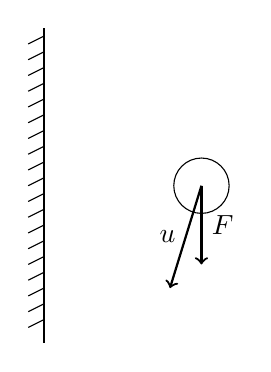
\begin{tikzpicture}
		\draw (-2,2) -- (-2,-2);
		\draw (-2.2, 1.8) -- (-2, 1.9);
		\draw (-2.2, 1.6) -- (-2, 1.7);
		\draw (-2.2, 1.4) -- (-2, 1.5);
		\draw (-2.2, 1.2) -- (-2, 1.3);
		\draw (-2.2, 1) -- (-2, 1.1);
		\draw (-2.2, 0.8) -- (-2, 0.9);
		\draw (-2.2, 0.6) -- (-2, 0.7);
		\draw (-2.2, 0.4) -- (-2, 0.5);
		\draw (-2.2, 0.2) -- (-2, 0.3);
		\draw (-2.2, 0) -- (-2, 0.1);
		\draw (-2.2,-1.8) -- (-2,- 1.7);
		\draw (-2.2,-1.6) -- (-2,- 1.5);
		\draw (-2.2,-1.4) -- (-2,- 1.3);
		\draw (-2.2,-1.2) -- (-2,- 1.1);
		\draw (-2.2,-1.0) -- (-2,- 0.9);
		\draw (-2.2,-0.8) -- (-2,- 0.7);
		\draw (-2.2,-0.6) -- (-2,- 0.5);
		\draw (-2.2,-0.4) -- (-2,- 0.3);
		\draw (-2.2,-0.2) -- (-2,- 0.1);
		\draw (0,0) circle (10pt);
		\draw [->,thick] (0,0) -- (-0.4,-1.3) node[left, midway] {$\bm{u}$};
		\draw [->, thick] (0,0) -- (0,-1) node[right, midway] {$\bm{F}$};
	\end{tikzpicture}

	Comparing with the original situation, we see there can be no lateral
	component of $\bm{u}$.
\end{eg}

\subsubsection{Forces balance}
Since there is no inertia, the forces must balance. From the equations,
\begin{equation}
	\nabla \cdot \sigma = - \bm{F} \implies \int_{\partial V} \sigma \cdot
	\bm{n} \,\diffd S + \int_V \bm{F} \,\diffd V = \bm{0}
\end{equation}

This is a consistency check on stress boundary conditions. 

Similarly, in the absence of fluid sources,
\begin{equation}
	\nabla \cdot \bm{u} = 0 \implies \int_{\partial V} \bm{u} \cdot \bm{n} \,
	\diffd S = 0
\end{equation}

This is a consistency check on velocity boundary conditions.

Likewise, torques balance, giving another consistency check on stress boundary
conditions.

\subsubsection{Work balances dissipation}
Intuitively, the flow has no kinetic energy (no inertia)  so any work done on
the fluid must be viscously dissipated instantaneously. We have
\begin{equation}
	\begin{aligned}
		\mathcal{D} &= 2\mu \int_V e_{ij} e_{ij} \, \diffd V \\
				&= \int (\sigma_{ij} + p \delta_{ij}) e_{ij} \, \diffd V \\
	&= \int \sigma_{ij} \frac{\partial u_i}{\partial x_j} + p e_{ii} \, \diffd V \\
	&= \int \frac{\partial}{\partial x_j} \sigma_{ij} u_i - u_i \frac{\partial
	\sigma_{ij}}{\partial x_j} \, \diffd V \\
	&= \int_{\partial V} \bm{u} \cdot \sigma \cdot \bm{n} \, \diffd S + \int
	\bm{u} \cdot \bm{F} \, \diffd V
	\end{aligned}
\end{equation}

The first term is the work done by surface forces at the boundary, and the
second term is the work done by body forces.

\subsection{Three Theorems Based on Dissipation Integrals}
\begin{lemma}
	\label{l1}
	If $\bm{u}^I$ is an incompressible flow and $\bm{u}^S$ is a Stokes flow
	with body force $\bm{F}^S$ then 
	\begin{equation}
		2\mu \int e^{I} : e^{S} \, \diffd V = \int_{\partial V} \bm{u}^I \cdot
		\sigma^S \cdot \bm{n} \, \diffd S + \int_V \bm{u}^I \cdot \bm{F}^S \,
		\diffd V
	\end{equation}
\end{lemma}
Proof. Same as `work balances dissipation'.

\begin{theorem}
	Uniqueness theorem. Suppose $\bm{u}_1, \bm{u}_2$ are Stokes flows with the
	same boundary conditions and body forces, i.e. $\bm{F}_1 = \bm{F}_2$ in
	$V$ and either $\bm{u}_1 = \bm{u}_2$ or $\sigma_1 \cdot \bm{n} = \sigma_2
	\cdot \bm{n}$ on $\partial V$. Then $\bm{u}_1 = \bm{u}_2$.
\end{theorem}

Proof. Let $\bm{u}^* = \bm{u}_1 - \bm{u}_2$. From lemma~\ref{l1}, 
\begin{equation}
	2\mu \int_V e^* : e^* \, \diffd V = 0
\end{equation}

Thus $e^* = 0$ in $V$. Hence we can deduce $\bm{u}^*$ consists entirely of
rigid body motion: $\bm{u}^* = \bm{U} + \bm{\Omega} \times \bm{u}$. Using the
boundary conditions, we have $\bm{U} = \bm{\Omega} = 0$ thus $\bm{u}_1 =
\bm{u}_2$, i.e. Stokes flows are unique.

\lecture{14/10/20}
\begin{theorem}
	Reciprocal theorem. If $\bm{u}_1$ and $\bm{u}_2$ are Stokes flows in $V$
	then
	\begin{equation}
		\int_{\partial V} \bm{u}_1 \cdot \sigma_2 \cdot \bm{n} \, \diffd S +
		\int_V \bm{u}_1 \cdot \bm{F}_2 \, \diffd V = 
		\int_{\partial V} \bm{u}_2 \cdot \sigma_1 \cdot \bm{n} \, \diffd S +
		\int_V \bm{u}_2 \cdot \bm{F}_1 \, \diffd V
	\end{equation}

	That is, work done by forces of flow 1 against flow 2 = work done by
	forces of flow 2 against flow 1.
\end{theorem}

Proof. Apply the lemma twice.

\begin{theorem}
	Minimum Dissipation theorem. Among all the incompressible flows in $V$
	that satisfy given velocity boundary conditions, the dissipation is
	minimised by the Stokes flow $\bm{u}^S$ with $\bm{F}^s = \bm{0}$
	satisfying the same velocity boundary conditions.
\end{theorem}

Proof. We have
\begin{equation}
	\begin{aligned}
		0 &\le 2\mu \int (e - e^S):(e-e^S) \, \diffd V \\
		  &\le 2\mu \int e:e - e^S:e^S \, \diffd V + 4\mu \int e^S : (e^S
		-e)\,\diffd V
	\end{aligned}
\end{equation}

Applying the lemma with $\bm{u}^I = \bm{u}^S - \bm{u}$, the last term is $0$
since $\bm{u}^I = 0$ on $\partial V$ and $\bm{F}^S = 0$ on $V$. Thus
\begin{equation}
	0 \le \mathcal{D} - \mathcal{D}^S
\end{equation}

\begin{eg}
	\begin{enumerate}
		\item Consider an irregularly shaped body in a Stokes flow with
			inscribing circle $S_1$ with radius $a_1$ and circumscribing
			circle $S_2$ with radius $a_2$. Suppose the body experiences a
			force $\bm{F}$ and has uniform velocity $\bm{U}$.
		\begin{center}
			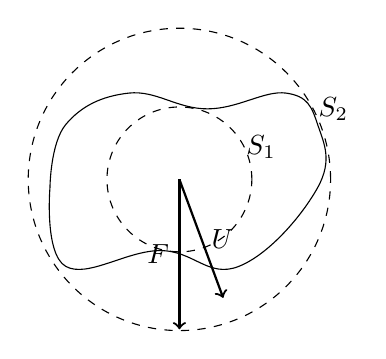
\begin{tikzpicture}[scale=0.4]
				\draw plot[smooth, tension=.7] coordinates {(-3.5, 0.5) (-3,
				2.5) (-1,3.5) (1.5,3) (4,3.5) (5,2.5) (5,0.5) (2.5,-2)
				(0,-1.5) (-3,-2) (-3.5,0.5)};
				\draw[dashed] (0.61,0.76) circle (2.3);
				\draw (5.5, 3) node {$S_2$};
				\draw[dashed] (0.61,0.76) circle (4.8);
				\draw (3.2, 1.8) node {$S_1$};
				\draw[thick, ->] (0.61,0.76) -- (0.61, -4) node [left, midway]
				{$\bm{F}$};
				\draw[thick, ->] (0.61,0.76) -- (2, -3) node [right, midway]
				{$\bm{U}$};
			\end{tikzpicture}
		\end{center}
		Applying the theorem by taking $\bm{U}^S$ to be the Stokes flow past
		$S_1$ and $\bm{U}^I$ to be the Stokes flow past $S_2$ superposed with
		solid body motion in the gap between $S_1$ and $S_2$, we have
		\begin{equation}
			(6\pi \mu a_1 U)U \le \bm{F} \cdot \bm{U} \le (6\pi \mu a_2 U)U
		\end{equation}

	\item Adding \emph{rigid} particles to a Stokes flow with given
		\emph{external} velocity boundary conditions increases dissipation
		and, if the particles are \emph{force-free} and \emph{torque-free},
		the apparent viscosity also increases.

		\begin{center}
			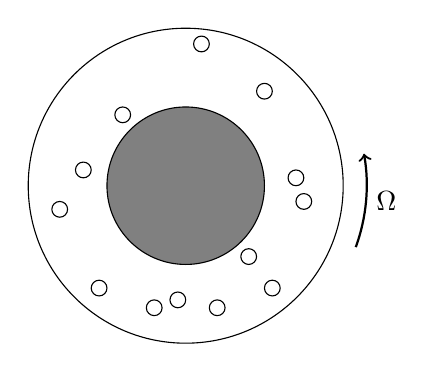
\begin{tikzpicture}
				\draw[fill=gray] (0,0) circle (1);
				\draw (0,0) circle (2);
				\draw (1.0, 1.2) circle (0.1);
				\draw (1.5, -0.2) circle (0.1);
				\draw (0.2, 1.8) circle (0.1);
				\draw (1.4, 0.1) circle (0.1);
				\draw (0.8, -0.9) circle (0.1);
				\draw (1.1, -1.3) circle (0.1);
				\draw (0.4, -1.55) circle (0.1);
				\draw (-0.1, -1.45) circle (0.1);
				\draw (-0.8, 0.9) circle (0.1);
				\draw (-1.1, -1.3) circle (0.1);
				\draw (-0.4, -1.55) circle (0.1);
				\draw (-1.3, 0.2) circle (0.1);
				\draw (-1.6, -0.3) circle (0.1);
				\draw[thick, ->] (2.16,-0.78) arc (-20:10:2.3)
				node[right,midway] {$\Omega$};
			\end{tikzpicture}
		\end{center}
	\item Inertia increases drag: consider $\rho \frac{\diffD \bm{u}}{\diffD
		t}$ as $\bm{F}$.
\end{enumerate}
\end{eg}

\subsection{Representation by Potentials}
Assume $\bm{F}$ = 0, or that $\bm{F}$ is conservative and absorbed by the
modified pressure. Consider the Stokes equations
\begin{align}
	\mu \nabla^2 \bm{u} &= \nabla p \label{stokes1} \\
	\nabla \cdot \bm{u} &= 0 \label{stokes2}
\end{align}

From these equations we have
\begin{equation}
	\begin{aligned}
		\nabla \cdot \eqref{stokes1} \& \eqref{stokes2} &\implies \nabla^2 p = 0 \implies
		p \hspace{.6em} \text{is harmonic} \\
		\nabla \times \eqref{stokes1} &\implies \nabla^2 \bm{\omega} = 0
		\implies \text{vorticity}\hspace{.6em}\bm{\omega} = \nabla \times
		\bm{u} \hspace{.6em} \text{is harmonic} \\
		\nabla^2  \eqref{stokes1} &\implies \nabla^4 \bm{u} = \bm{0} \implies
		\bm{u} \hspace{.6em} \text{is \emph{bi-harmonic}}
	\end{aligned}
\end{equation}

In two dimensions, we can use a stream-function so that $\bm{u} = \nabla
\times (0,0,\psi)$. Then
\begin{equation}
	\omega_z = -\nabla^2 \psi \implies \nabla^4 \psi = 0
\end{equation}

Similarly, in axisymmetric spherical polars, $\bm{u} = \nabla \times
(0,0,\frac{\Psi}{r \sin \theta})$. Then $\omega_\phi = -\frac{E^2 \Psi}{r\sin
\theta}$ and $E^4 \Psi = 0$ where
\begin{equation}
	E^2 = \frac{\partial^2}{\partial r^2} + \frac{\sin \theta}{r^2}
	\frac{\partial}{\partial \theta} \left( \sin \theta
	\frac{\partial}{\partial \theta}\right)
\end{equation}

Many exact solutions can be found in coordinate systems where the operators
$\nabla^2, \nabla^4, E^2$, etc are separable.

\subsection{Complex Variable Theory in 2D Flow}
Writing $z = x+iy, \bar{z} = x-iy$ gives
\begin{equation}
	\nabla^2 = 4 \frac{\partial^2}{\partial z \partial \bar{z}}
\end{equation}
Thus $f(x,y)$ analytic implies $f = f(z)$ or equivalently $\frac{\partial
f}{\partial \bar{z}} = 0$. Thus $\Re f$ and $\Im f$ are harmonic.

Similarly $\nabla^4 \psi = 0$ implies $\psi$ can be written as $\psi =
\Im(\bar{z}\phi + \chi)$ where $\phi(z), \chi(z)$ are analytic.

We can find clever exact solutions to difficult problems using this theory,
but it is limited to 2D.

\subsection{Papkovich-Neuber Solution}
Let $p = \nabla^2 \pi$ where
\begin{equation}
	\pi(\bm{x}) = -\frac{1}{4\pi} \int \frac{p(\bm{x'})}{\left|
	\bm{x}-\bm{x'}\right|} \, \diffd V
\end{equation}

Then the Stokes equations can be written $\nabla^2 \left( \mu \bm{u} - \nabla
\pi\right) = 0$. Thus
\begin{equation}
	\mu \bm{u} = \nabla \pi - \bm{\Phi}
\end{equation}
where $\nabla^2 \bm{\Phi} = 0$. Now $\nabla \cdot \bm{u} = 0$ implies
$\nabla^2 \pi = \nabla \cdot \bm{\Phi}$. Then
\begin{equation}
	\pi = \frac{1}{2}\left(\bm{x}\cdot\bm{\Phi} + \chi\right)
\end{equation}
where $\nabla^2 \psi = 0$. Thus \emph{any} Stokes flow with $\bm{F} = 0$ can
be written in terms of a harmonic vector $\bm{\Phi}$ and a harmonic scalar
$\chi$. The Stokes equations are then
\begin{equation}
	\begin{aligned}
		2\mu \bm{u} &= \nabla \left(\bm{x} \cdot \bm{\Phi} + \chi\right) -
	2\bm{\Phi} \\
	p &= \nabla \cdot \bm{\Phi}
\end{aligned}
\end{equation}
which may also be re-written with the $2\mu$ factor absorbed by $p$.

Note the following.
\begin{enumerate}
	\item Any irrotational flow $2 \mu \bm{u} = \nabla \chi$ is also a Stokes
		flow, though $p = 0$ and $\dunder{\sigma} = \nabla \nabla \chi$ which
		is different from an inviscid irrotational flow.
	\item It is sometimes possible to find a harmonic scalar $\phi$ with
		$\chi = \bm{x} \cdot \nabla \phi - 2 \phi$. If so, $\chi$ can be
		eliminated by writing $\bm{\Phi}' = \bm{\Phi} + \nabla \phi$. For
		example, if $\chi$ has a spherical harmonic expansion we can eliminate
		all of the terms except the uniform strain $\chi/2\mu = \frac{1}{2}
		\bm{x} \cdot \dunder{E} \cdot \bm{x} \iff \bm{u} = \dunder{E} \cdot
		\bm{x}$, since $\chi = r^n Y_n^m(\theta,\phi) \iff \phi =
		\frac{r^n}{n-2} Y_n^m(\theta,\phi)$ which fails for $n=2$.
	\item Conversely, if $\bm{\Phi} = \nabla \phi$ then we can get the same
		$\bm{u}$ from $\chi = \bm{x} \cdot \nabla \phi - 2\phi$, which is
		easier to calculate.
\end{enumerate}

\subsection{Solutions for points, spheres (and cylinders)}
A point or sphere has no intrinsic direction or orientation, thus solutions on
these geometries should also have no intrinsic direction or orientation.

\subsubsection{Spherical harmonic functions}
Let $r = \abs{\x}$. Recall $\nabla^2 (\frac{1}{r}) = 0$ for $r \ne 0$. All
other spherical harmonic functions $\phi$ with $\phi \to 0$ as $r \to \infty$
are obtained from 
\begin{equation}
	\frac{1}{r}, \hspace{1em}\nabla \frac{1}{r},\hspace{1em} \nabla \nabla
	\frac{1}{r}, \hspace{1em}\text{etc.}
\end{equation}
The harmonic functions which are bounded as $r \to 0$ are
obtained from 
\begin{equation}
	r \cdot \inv{r} = 1,\hspace{1em} r^3 \nabla \inv{r} = -\x,\hspace{1em} r^5 \nabla
\nabla \inv{r},\hspace{1em} \dots,\hspace{1em} r^{2n+1} \nabla^n \inv{r}
\end{equation}

Compare with separable solutions, for example the $2n+1$ solutions in
spherical polars given by
\begin{equation}
\begin{pmatrix} r^n \\ r^{-n-1} \end{pmatrix} P_n^m(\theta) \begin{pmatrix}
\cos m \phi \\ \sin m\phi\end{pmatrix}
\end{equation}
where $P_n^m$ are \emph{associated Legendre functions} and $0 \le m \le n$.


Recall the following results.
\begin{equation}
	\begin{aligned}
		\nabla \x &= \dunder{I} \\
		\nabla r &= \frac{\x}{r} \\
		\nabla f(r) &= f'(r) \nabla r = f'(r) \frac{\x}{r}
	\end{aligned}
\end{equation}

Hence we have
\begin{equation}
	\begin{aligned}
		\nabla \inv{r} &= -\frac{\x}{r^3} \\
		\nabla \nabla \inv{r} &= -\frac{\dunder{I}}{r^3} +
		\frac{3\x\cdot\x}{r^5} \\
		\nabla_i \nabla_j \nabla_k \inv{r} &= \nabla_i \left(
		-\frac{\delta_{jk}}{r^3} + \frac{3x_j\cdot x_k}{r^5}\right)\\
		&= \frac{3(x_i \delta_{jk} + x_j \delta_{ik} + x_k \delta_{ij})}{r^5}
		- \frac{15 x_i x_j x_k}{r^7}
	\end{aligned}
\end{equation}

Note: these depend only on $\x$ and $r$ and thus have no preferred direction,
as hoped. We can use these functions to form Papkovich-Neuber potentials
$\bm{\Phi}$ and $\chi$ by multiplying the harmonic functions above by constant
scalars, vectors or tensors and taking an appropriate number of dot products,
e.g. the following are all harmonic vectors
\begin{equation}
	\bm{A} \inv{r}, \hspace{1em} \dunder{B} \cdot \nabla \inv{r},
	\hspace{1em} C \nabla \inv{r}, \hspace{1em} (\bm{D} \cdot \nabla)\nabla
	\inv{r}, \hspace{1em} (\dunder{E}:\nabla\nabla)\nabla\inv{r}, \hspace{1em}
	\bm{\Omega} \times \nabla \inv{r}
\end{equation}

It is useful to distinguish between \emph{true} and \emph{pseudo} tensors.
True / pseudo tensors keep / change sign upon reflection, e.g.
\begin{equation}
	T_{ijk}' = \pm R_{il} R_{jm} R_{kn} T_{lmn}
\end{equation}

Examples of true vectors are velocity $\bm{u}$; force $\bm{F}$; position $\x$;
 del $\nabla$; identity $\dunder{I}$.
Examples of pseudo vectors are angular velocity $\bm{\Omega}$; torque
$\bm{G}$; $\bm{u} \times \x$; vorticity $\bm{\omega} = \nabla \times \bm{u}$.
Products obey the obvious parity rules, e.g. helicity $\bm{u} \cdot
\bm{\Omega}$ is a pseudo scalar.

\subsection{Solution due to a point force}
The Papkovich-Neuber solution due to a point force is a Green's function for
the Stokes equations. This problem is also known as a `Stokeslet'. Consider
the problem
\begin{equation}
	\begin{aligned}
		\nabla \cdot \dunder{\sigma} &= \mu \nabla^2 \bm{u} - \nabla p = -
		\bm{F} \delta(\x) \\
		\nabla \cdot \bm{u} &= 0
	\end{aligned}
\end{equation}
with $\bm{u} \to 0$ at infinity. The answer must be linear in $\bm{F}$, but
otherwise has no orientation. The only choice is $\bm{\Phi} = \alpha
\frac{\bm{F}}{r}$. We could have tried $\bm{F} \times \nabla \inv{r}$, but
this is a pseudo vector whilst $\bm{\Phi}$ and $\chi$ need to be true since
$\bm{u}$ is true. Similar arguments rule out other harmonic functions.

\lecture{19/10/20}
We have
\begin{equation}
	\begin{aligned}
		2\mu \bm{u} &= \alpha \left( \nabla \left( \frac{\bm{F} \cdot
			\x}{r}\right) - 2
		\frac{\bm{F}}{r}\right) \\
		&= \alpha \left( \frac{\bm{F} \cdot \dunder{I}}{r} -
	\frac{(\bm{F}\cdot\x)\x}{r^3} - 2\frac{\bm{F}}{r}\right) \\
	&= -\alpha \left( \frac{\bm{F}}{r} + \frac{(\bm{F}\cdot\x)\x}{r^3}\right)
\end{aligned}
\end{equation}

Thus the stress tensor is
\begin{equation}
	\dunder{\sigma} = \mu \left( \nabla \bm{u} + \nabla \bm{u}^T\right) -
	\left(\nabla \cdot \bm{\Phi}\right)\dunder{I} = 3\alpha (\bm{F} \cdot
	\bm{x}) \frac{\x \x}{r^5}
\end{equation}

On any sphere $r=R$, $\bm{n} = \frac{\x}{R}$, and
\begin{equation}
	\begin{aligned}
		2\mu \bm{u}\cdot\bm{n} &= -\frac{2\alpha}{R} \bm{F}\cdot\bm{n} \\
		\dunder{\sigma} \cdot \bm{n} &= 3 \alpha \frac{(\bm{F} \cdot
		\bm{n}) \bm{n}}{R^2}
	\end{aligned}
\end{equation}

To determine the constant $\alpha$ we can consider the surface volume flux and
the surface stress. The surface volume flux is
\begin{equation}
	\int_{r=R} \bm{u}\cdot\bm{n}\,\diffd S = -\frac{\alpha \bm{F}}{\mu R}
	\cdot \int_{r=R} \bm{n} \, \diffd S = 0
\end{equation}
which does not provide any information on $\alpha$. The surface forces should
equal $-\bm{F}$. We have
\begin{equation}
	-\bm{F} = \int_{r=R} \dunder{\sigma} \cdot \bm{n} \, \diffd S = 3\alpha
	\bm{F} \cdot \int_{r=R} \bm{n} \bm{n} \, \frac{\diffd S}{R^2} = 3 \alpha
	\bm{F} \cdot \frac{4\pi}{3} \dunder{I} = 4\pi \alpha \bm{F}
\end{equation}

Hence we choose $\alpha = -1/4\pi$. Thus the final solution is
\begin{equation}
	\bm{u} = \bm{F} \cdot \dunder{J}(\x), \hspace{2em} \dunder{\sigma} =
	\bm{F} \cdot \dunder{\underline{K}}(\x), \hspace{2em} p =
	\frac{\bm{F}\cdot\x}{4\pi r^3}
\end{equation}
where $\dunder{J}$ is the \emph{Oseen tensor}:
\begin{equation}
	\dunder{J} = \frac{1}{8\pi \mu} \left( \frac{\dunder{I}}{r} +
		\frac{\x\x}{r^3}\right), \hspace{2em} \dunder{\underline{K}} =
		-\frac{3}{4\pi} \frac{\x\x\x}{r^5}
\end{equation}

Finally, from incompressibility $\nabla \cdot \bm{u} = 0$ and the Stokes
equations $\nabla \cdot \dunder{\sigma} = -\bm{F}\delta(\x)$, we deduce
\begin{equation}
	\nabla \cdot \dunder{J} = 0, \hspace{2em} \nabla \cdot
	\dunder{\underline{K}} = - \dunder{I}\delta(\x)
\end{equation}

Note that the velocity scales as $u \propto \inv{r}$: see
figure~\ref{fig:stokeslet}. This is slowly decaying compared to many forces
e.g. gravity which scales as $\inv{r^2}$. Thus particle interactions in Stokes
flow can occur on much larger scales than (for example) charge interactions.

\begin{figure}
\begin{center}
	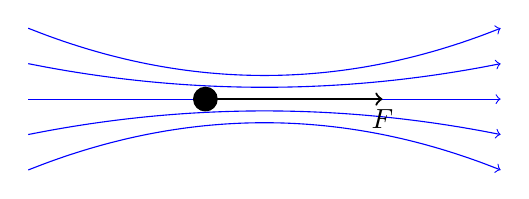
\begin{tikzpicture}[scale=1.5]
	\draw[smooth,domain=-2:2,blue,->] plot({\x},{0.05*\x*\x+0.1});
	\draw[smooth,domain=-2:2,blue,->] plot({\x},{0.1*\x*\x+0.2});
	\draw[smooth,domain=-2:2,blue,->] plot({\x},{-0.1*\x*\x-0.2});
	\draw[smooth,domain=-2:2,blue,->] plot({\x},{-0.05*\x*\x-0.1});
	\draw[smooth,domain=-2:2,blue,->] plot({\x},{0});
	\draw[fill=black] (-0.5,0) circle (0.1);
	\draw[thick,->] (-0.5, 0) -- (1, 0) node[below] {$\bm{F}$};
\end{tikzpicture}
\end{center}
\caption{Stokeslet solution for a point force.}
\label{fig:stokeslet}
\end{figure}

\subsection{Source flow}
Consider a source of strength $Q$ with $\nabla \cdot \bm{u} = Q \delta(\x)$.
This is reffered to as a \emph{point volume source}. One can show the solution
is
\begin{equation}
	\bm{u} = \frac{Q\x}{4\pi r^3}
\end{equation}
which is obtained using Papkovich-Neuber potentials
\begin{equation}
	\chi = \alpha \frac{Q}{r}, \hspace{2em} \bm{\Phi} = \beta Q \nabla \inv{r}
\end{equation}

\subsection{Force dipole, stresslet, rotlet}
Further solutions for dipoles, quadrupoles, etc. can be found by taking
gradients of the Stokeslet and source solutions. For example, consider a
dipole.

\begin{center}
	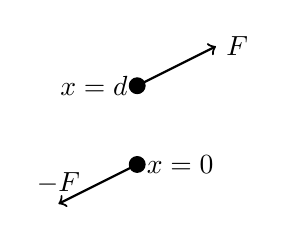
\begin{tikzpicture}
		\draw[fill] (0,0) circle (0.1) node[right] {$\x = \bm{0}$};
		\draw[fill] (0,1) circle (0.1) node[left] {$\x = \bm{d}$};
		\draw[thick, ->] (0,0) -- (-1,-0.5) node[above] {$-\bm{F}$};
		\draw[thick, ->] (0,1) -- (1, 1.5) node[right] {$\bm{F}$};
	\end{tikzpicture}
\end{center}

The Stokeslet solution is
\begin{equation}
	\bm{u} = \bm{F}\cdot\dunder{J} (\x-\bm{d}) - \bm{F} \cdot \dunder{J}(\x) =
	\bm{F} \cdot (-\bm{d}\cdot\nabla)\dunder{J}(\x) + \text{h.o.t.}
\end{equation}

Take the limit $\bm{d} \to \bm{0}$ with $\bm{F}\bm{d}$ fixed and split $-F_i
d_j$ into
\begin{enumerate}
	\item An isotropic part $-\frac{1}{3} F_k d_k \delta_{ij}$
	\item A symmetric traceless part
		\begin{equation}
			s_{ij} = -\frac{1}{2} (F_i d_j + F_j d_i) + \frac{1}{3} F_k d_k
			\delta_{ij}
		\end{equation}
	\item An antisymmetric part $-\frac{1}{2}\varepsilon_{ijk} G_k$ where
		$\bm{G} = \bm{d} \times \bm{F}$
\end{enumerate}

The flow contribution from each of these components may then be calculated.
\begin{enumerate}
	\item The isotropic component gives no flow since $\nabla \cdot \dunder{J}
		= 0$
	\item This component is a \emph{stresslet} representing the following
		components of motion
		\begin{center}
			\begin{tikzpicture}[scale=0.7]
				\draw[fill] (0,1) circle (0.1);
				\draw[fill] (0,-1) circle (0.1);
				\draw[thick,->] (0,2) -- (0,1.1) node[right] {$\bm{F}$};
				\draw[thick,->] (0,-2) -- (0,-1.1) node[right] {$-\bm{F}$};
				\draw[fill] (-7,0) circle (0.1);
				\draw[fill] (-5,0) circle (0.1);
				\draw[thick,->] (-7,0) -- (-8,0) node[left] {$-\bm{F}$};
				\draw[thick,->] (-5,0) -- (-4,0) node[right] {$\bm{F}$};
				\draw[fill] (7,0) circle (0.1);
				\draw[fill] (5,0) circle (0.1);
				\draw[fill] (6, 1) circle (0.1);
				\draw[fill] (6, -1) circle (0.1);
				\draw[thick,->] (7,0) -- (7.8, 0) node[right] {$\bm{F}/2$};
				\draw[thick,->] (5,0) -- (4.2, 0);
				\draw[thick,->] (6, 1.9) -- (6,1.1);
				\draw[thick,->] (6,-1.9) -- (6,-1.1);
			\end{tikzpicture}
		\end{center}

	\item This component is a \emph{rotlet} due to a point torque $\bm{G}$.
		\begin{center}
			\begin{tikzpicture}
				\draw[fill] (0,0.5) circle (0.1);
				\draw[fill] (0,-0.5) circle (0.1);
				\draw[thick,->] (0,0.5) -- (-1, 0.5);
				\draw[thick,->] (0,-0.5) -- (1, -0.5);
				\draw[fill] (4, 0) circle (0.1);
				\draw[fill] (5, 0) circle (0.1);
				\draw[thick,->] (4,0) -- (4,1);
				\draw[thick,->] (5,0) -- (5,-1);
			\end{tikzpicture}
		\end{center}
\end{enumerate}

Both the stresslet and rotlet decay as $\inv{r^2}$.

\subsection{Rigid sphere with velocity U}
Consider a rigid sphere of radius $a$ moving uniformly  with velocity
$\bm{U}$ in a Stokes flow. We have $\nabla \cdot \bm{u} = 0$ and $\mu \nabla^2
\bm{u} = \nabla p$ in $r > a$. We require $\bm{u} \to 0$ as $r \to \infty$ and
$\bm{u} = \bm{U}$ on the sphere's surface $r=a$. The sphere is isotropic, so
we need harmonic functions of $\x, \bm{U}$ which are linear in $\bm{U}$; decay
at $\infty$; and are true tensors. We choose
\begin{equation}
	\frac{1}{2\mu} \bm{\Phi} = \alpha \bm{U} \inv{r}, \hspace{2em}
	\frac{1}{2\mu} \chi = \beta \bm{u} \cdot \nabla \inv{r}
\end{equation}

This gives a solution which is a superposition of a Stokeslet and a source
dipole
\begin{equation}
	\bm{u} = -\alpha \left( \frac{\bm{U}}{r} +
		\frac{(\bm{U}\cdot\x)\x}{r^3}\right) + \beta \left(
	-\frac{\bm{U}}{r^3} + 3 \frac{(\bm{U}\cdot\x)\x}{r^5}\right)
\end{equation}

Enforcing the boundary condition $\bm{u} = \bm{U}$ on $r=a$ requires
\begin{equation}
	\begin{aligned}
		-\frac{\alpha}{a} - \frac{\beta}{a^3} &= 1, \hspace{2em}
		-\frac{\alpha}{a} + 3 \frac{\beta}{a^3} = 0 \\
		\implies \alpha &= -\frac{3a}{4}, \hspace{1em} \beta = -\frac{a^3}{4}
	\end{aligned}
\end{equation}

Thus the final solution for a sphere in a Stokes flow is
\begin{equation}
	\bm{u} = \frac{3}{4}\bm{U}\left(\frac{a}{r} + \frac{a^3}{3r^3} \right) +
	\frac{3}{4} \frac{(\bm{U}\cdot\x)\x}{r^2} \left( \frac{a}{r} -
	\frac{a^3}{r^3}\right)
\end{equation}

The corresponding pressure and vorticity, both of which are harmonic and due
to the Stokeslet, are
\begin{equation}
	p = \frac{3}{2}\mu a \frac{\bm{U}\cdot\x}{r^3}, \hspace{2em}\bm{\omega} =
	-\frac{1}{\mu} \nabla \times \bm{\Phi} = \frac{3a}{2}\frac{\bm{U} \times
	\bm{x}}{r^3}
\end{equation}


\end{document}
